

\begin{wrapfigure}[0]{r}[-2cm]{4cm}
 \vspace{-5cm}
 %\centering 
 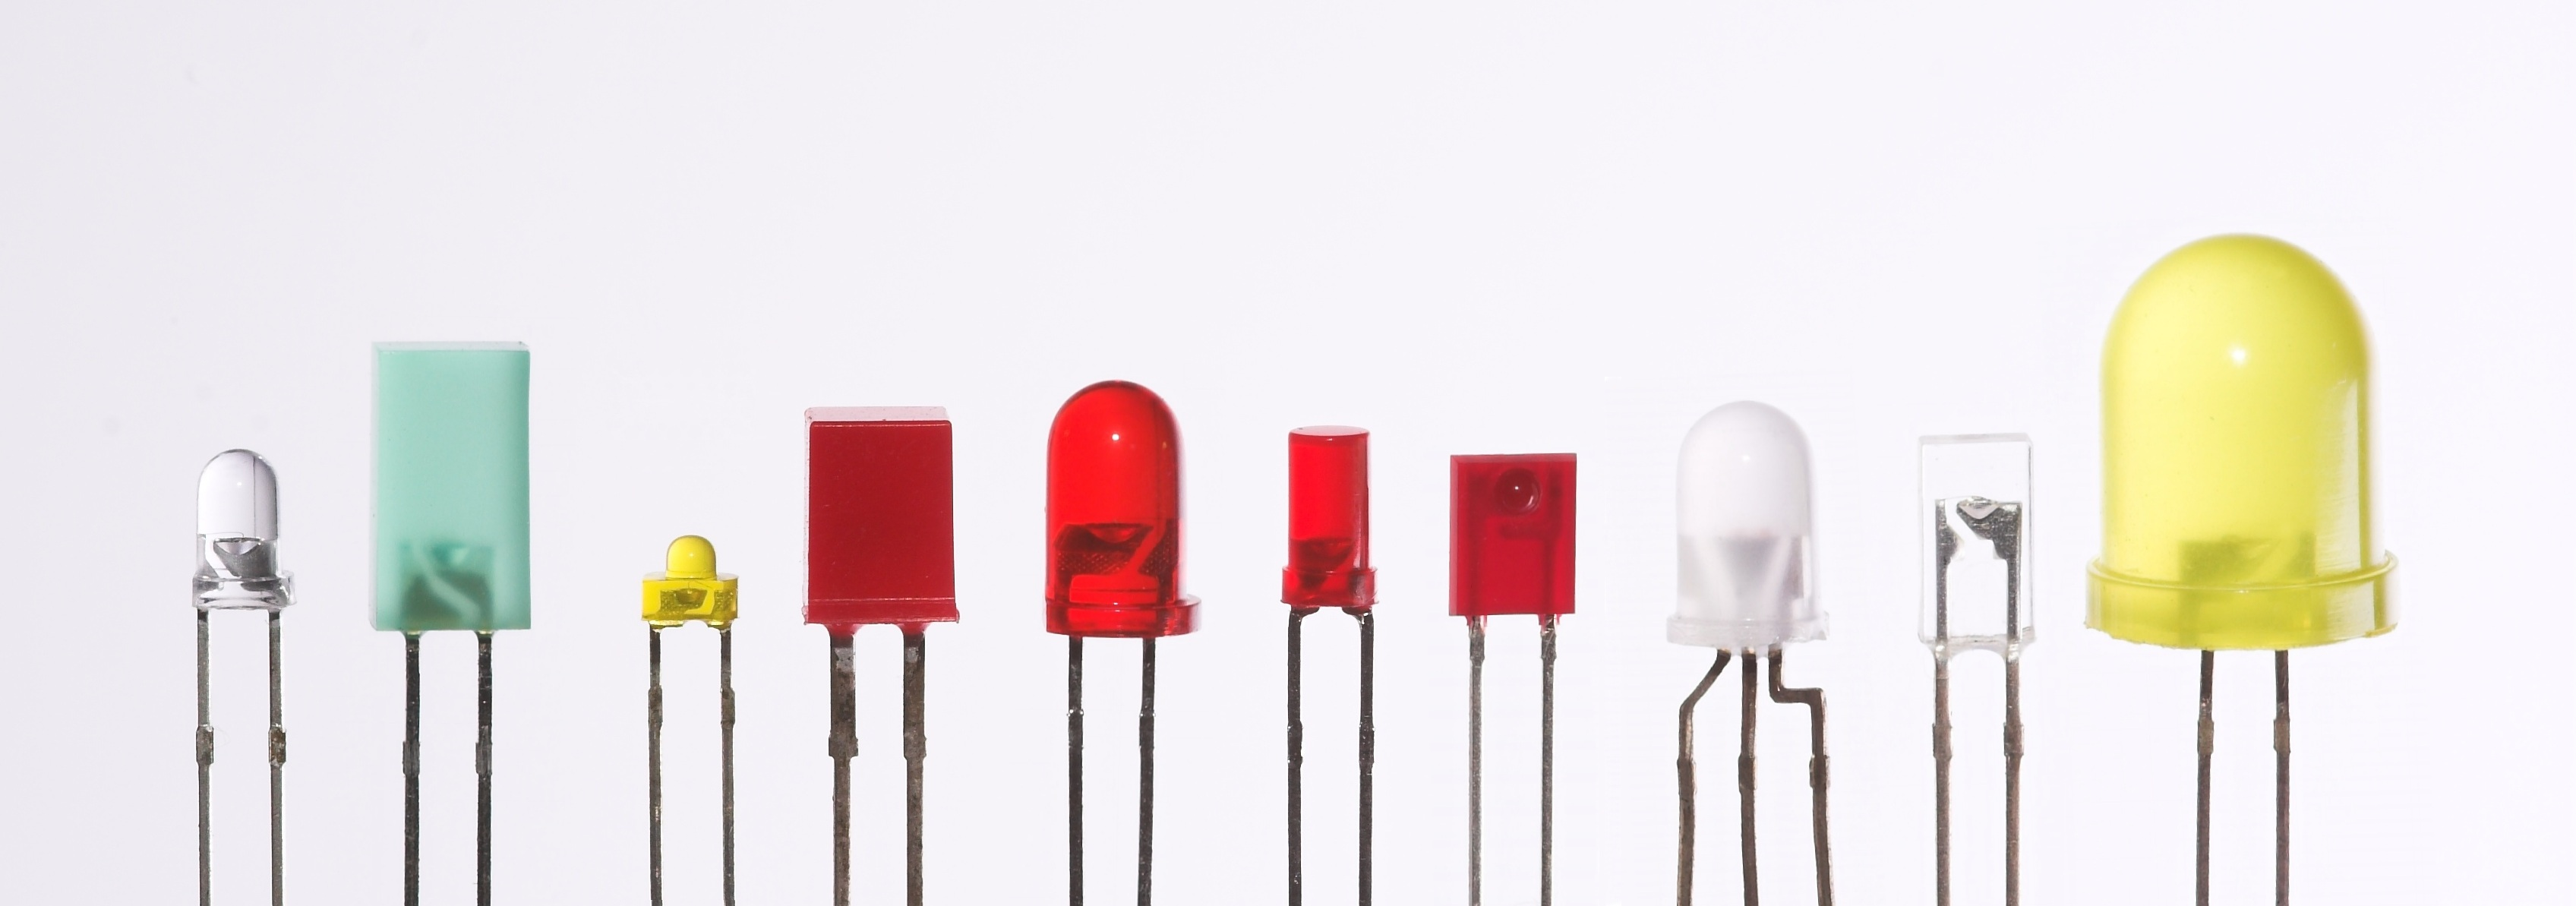
\includegraphics[scale=0.25]{Diode/Bilder/Verschiedene_LEDs.jpg}
 %\caption{Bildunterschrift der Grafik.}
 %\label{fig:meine-Grafik}
 \vspace*{-5cm}
\end{wrapfigure}


\section{Theorie- und Prüfungsfragen} 

\subsection*{Dotierung}

\begin{enumerate}
	\itemsep1pt\parskip0pt\parsep0pt
	\item[i] Was bedeutet der Begriff Dotierung?
\end{enumerate}

\begin{enumerate}
\item[ii] \emph{\textbf{TB105}}    Was verstehen Sie unter Halbleitermaterialien? Einige Stoffe wie z.B. ...
	\begin{enumerate}
	\itemsep1pt\parskip0pt\parsep0pt
		\item[a] Silizium, Germanium sind in reinem Zustand gute Isolatoren. Durch geringfügige Zusätze von geeigneten anderen Stoffen werden sie jedoch zu Leitern.
		\item[b] Silizium, Germanium sind in reinem Zustand gute Isolatoren. Durch geringfügige Zusätze von geeigneten anderen Stoffen nimmt jedoch ihre Leitfähigkeit ab.
		\item[c]  Indium oder Magnesium sind in reinem Zustand gute Isolatoren. Durch geringfügige Zusätze von geeigneten anderen Stoffen werden sie jedoch zu Leitern.
		\item[d] Silizium, Germanium sind in trockenem Zustand gute Elektrolyten. Durch geringfügige Zusätze von Wismut oder Tellur kann man daraus entweder N-leitendes oder P-leitendes Material für Anoden bzw. Katoden von Halbleiterbauelementen herstellen.
	\end{enumerate}
\end{enumerate}

\begin{enumerate}
\item[iii] \emph{\textbf{TC501}}    P-dotiertes Halbleitermaterial ist solches, das mit einem zusätzlichen Stoff versehen wurde, der
	\begin{enumerate}
	\itemsep1pt\parskip0pt\parsep0pt
		\item[a] mehr als vier Valenzelektronen enthält.
		\item[b] genau vier Valenzelektronen enthält.
		\item[c] weniger als vier Valenzelektronen enthält.
		\item[d] keine Valenzelektronen enthält.
	\end{enumerate}
\end{enumerate}


\begin{enumerate}
\item[iv] \emph{\textbf{TC502}}   N-leitendes Halbleitermaterial ist gekennzeichnet durch
	\begin{enumerate}
	\itemsep1pt\parskip0pt\parsep0pt
		\item[a] Überschuss an freien Elektronen.
		\item[b] das Fehlen von Dotierungsatomen.
		\item[c] das Fehlen von Atomen im Gitter des Halbleiterkristalls.
		\item[d] das Fehlen von Atomen im Gitter des Halbleiterkristalls.
	\end{enumerate}
\end{enumerate}


\begin{enumerate}
\item[v] \emph{\textbf{TC503}}  Ein in Durchlassrichtung betriebener PN-Übergang ermöglicht
	\begin{enumerate}
	\itemsep1pt\parskip0pt\parsep0pt
		\item[a] den Stromfluss von N nach P.
		\item[b] den Stromfluss von P nach N.
		\item[c] keinen Stromfluss.
		\item[d] den Elektronenfluss von P nach N.
	\end{enumerate}
\end{enumerate}


\loesung{
	\begin{enumerate}
		\item[i] \textbf{Dotierung} bezeichnet in der Halbleitertechnik das einbringen von Fremdatomen in ein Grundmaterial zur Veränderung der elektrischen Leitfähigkeit.
		\item[ii]  a
		\item[iii] c
		\item[iv]  a
		\item[v] b
	\end{enumerate}
}



\subsection*{Die Diode}

\begin{enumerate}
\itemsep1pt\parskip0pt\parsep0pt
\item[vi] Skizziere das Schaltzeichen einer Diode und markieren die Anode und die Kathode und die jeweilige Dotierung.
\item[vii] Skizziere die Strom-Spannungskennlinie und markieren den Durchlassbereich, den Sperrbereich und den Durchbruchbereich.
\item[viii] Skizziere das Schaltzeichen einer Zener-Diode?
\item[iv] Skizziere eine Schaltung mit deren Hilfe eine Spannungsstabilisierung durchgeführt werden kann.
\end{enumerate}

\loesung{
\begin{figure}[H]
	\centering
	\subfigure[vi]{% Graphic for TeX using PGF
% Title: /home/stole/Dokumente/git/afutub-kurs/Praxisskript/Diode/Schaltungen/Diode.dia
% Creator: Dia v0.97.3
% CreationDate: Mon Nov 16 20:36:17 2015
% For: stole
% \usepackage{tikz}
% The following commands are not supported in PSTricks at present
% We define them conditionally, so when they are implemented,
% this pgf file will use them.
\ifx\du\undefined
  \newlength{\du}
\fi
\setlength{\du}{15\unitlength}
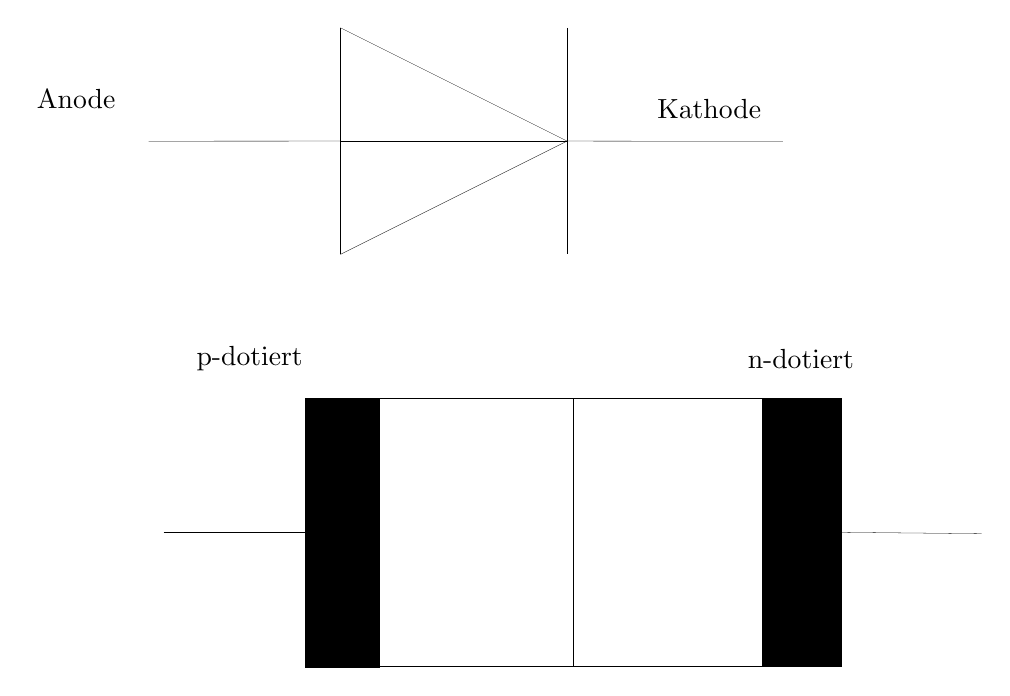
\begin{tikzpicture}
\pgftransformxscale{1.000000}
\pgftransformyscale{-1.000000}
\definecolor{dialinecolor}{rgb}{0.000000, 0.000000, 0.000000}
\pgfsetstrokecolor{dialinecolor}
\definecolor{dialinecolor}{rgb}{1.000000, 1.000000, 1.000000}
\pgfsetfillcolor{dialinecolor}
\pgfsetlinewidth{0.100000\du}
\pgfsetdash{}{0pt}
\pgfsetdash{}{0pt}
\pgfsetbuttcap
\pgfsetmiterjoin
\pgfsetbuttcap
\pgfsetmiterjoin
\pgfsetdash{}{0pt}
\definecolor{dialinecolor}{rgb}{0.000000, 0.000000, 0.000000}
\pgfsetstrokecolor{dialinecolor}
\draw (15.422302\du,-15.899999\du)--(15.422302\du,-13.022298\du);
\pgfsetbuttcap
\pgfsetmiterjoin
\pgfsetdash{}{0pt}
\definecolor{dialinecolor}{rgb}{0.000000, 0.000000, 0.000000}
\pgfsetstrokecolor{dialinecolor}
\draw (15.422302\du,-13.022298\du)--(18.300002\du,-14.461149\du);
\pgfsetbuttcap
\pgfsetmiterjoin
\pgfsetdash{}{0pt}
\definecolor{dialinecolor}{rgb}{0.000000, 0.000000, 0.000000}
\pgfsetstrokecolor{dialinecolor}
\draw (15.422302\du,-15.899999\du)--(18.300002\du,-14.461149\du);
\pgfsetbuttcap
\pgfsetmiterjoin
\pgfsetdash{}{0pt}
\definecolor{dialinecolor}{rgb}{0.000000, 0.000000, 0.000000}
\pgfsetstrokecolor{dialinecolor}
\draw (15.422302\du,-14.461149\du)--(18.300002\du,-14.461149\du);
\pgfsetbuttcap
\pgfsetmiterjoin
\pgfsetdash{}{0pt}
\definecolor{dialinecolor}{rgb}{0.000000, 0.000000, 0.000000}
\pgfsetstrokecolor{dialinecolor}
\draw (18.300002\du,-15.899999\du)--(18.300002\du,-13.022298\du);
\pgfsetlinewidth{0.100000\du}
\pgfsetdash{}{0pt}
\pgfsetdash{}{0pt}
\pgfsetbuttcap
{
\definecolor{dialinecolor}{rgb}{0.000000, 0.000000, 0.000000}
\pgfsetfillcolor{dialinecolor}
% was here!!!
\definecolor{dialinecolor}{rgb}{0.000000, 0.000000, 0.000000}
\pgfsetstrokecolor{dialinecolor}
\draw (18.300002\du,-14.461149\du)--(21.040301\du,-14.459230\du);
}
\pgfsetlinewidth{0.100000\du}
\pgfsetdash{}{0pt}
\pgfsetdash{}{0pt}
\pgfsetbuttcap
{
\definecolor{dialinecolor}{rgb}{0.000000, 0.000000, 0.000000}
\pgfsetfillcolor{dialinecolor}
% was here!!!
\definecolor{dialinecolor}{rgb}{0.000000, 0.000000, 0.000000}
\pgfsetstrokecolor{dialinecolor}
\draw (12.987653\du,-14.460276\du)--(15.422302\du,-14.461149\du);
}
% setfont left to latex
\definecolor{dialinecolor}{rgb}{0.000000, 0.000000, 0.000000}
\pgfsetstrokecolor{dialinecolor}
\node[anchor=west] at (11.448825\du,-14.995418\du){Anode};
% setfont left to latex
\definecolor{dialinecolor}{rgb}{0.000000, 0.000000, 0.000000}
\pgfsetstrokecolor{dialinecolor}
\node[anchor=west] at (19.327825\du,-14.872736\du){Kathode};
\pgfsetlinewidth{0.100000\du}
\pgfsetdash{}{0pt}
\pgfsetdash{}{0pt}
\pgfsetmiterjoin
\definecolor{dialinecolor}{rgb}{1.000000, 1.000000, 1.000000}
\pgfsetfillcolor{dialinecolor}
\fill (14.976770\du,-11.192971\du)--(14.976770\du,-7.792972\du)--(18.376770\du,-7.792972\du)--(18.376770\du,-11.192971\du)--cycle;
\definecolor{dialinecolor}{rgb}{0.000000, 0.000000, 0.000000}
\pgfsetstrokecolor{dialinecolor}
\draw (14.976770\du,-11.192971\du)--(14.976770\du,-7.792972\du)--(18.376770\du,-7.792972\du)--(18.376770\du,-11.192971\du)--cycle;
\pgfsetlinewidth{0.100000\du}
\pgfsetdash{}{0pt}
\pgfsetdash{}{0pt}
\pgfsetmiterjoin
\definecolor{dialinecolor}{rgb}{1.000000, 1.000000, 1.000000}
\pgfsetfillcolor{dialinecolor}
\fill (18.376770\du,-11.192970\du)--(18.376770\du,-7.792971\du)--(21.776770\du,-7.792971\du)--(21.776770\du,-11.192970\du)--cycle;
\definecolor{dialinecolor}{rgb}{0.000000, 0.000000, 0.000000}
\pgfsetstrokecolor{dialinecolor}
\draw (18.376770\du,-11.192970\du)--(18.376770\du,-7.792971\du)--(21.776770\du,-7.792971\du)--(21.776770\du,-11.192970\du)--cycle;
\pgfsetlinewidth{0.100000\du}
\pgfsetdash{}{0pt}
\pgfsetdash{}{0pt}
\pgfsetbuttcap
{
\definecolor{dialinecolor}{rgb}{0.000000, 0.000000, 0.000000}
\pgfsetfillcolor{dialinecolor}
% was here!!!
\definecolor{dialinecolor}{rgb}{0.000000, 0.000000, 0.000000}
\pgfsetstrokecolor{dialinecolor}
\draw (13.176770\du,-9.492971\du)--(14.976770\du,-9.492972\du);
}
\pgfsetlinewidth{0.100000\du}
\pgfsetdash{}{0pt}
\pgfsetdash{}{0pt}
\pgfsetmiterjoin
\definecolor{dialinecolor}{rgb}{0.000000, 0.000000, 0.000000}
\pgfsetfillcolor{dialinecolor}
\fill (14.976770\du,-11.192971\du)--(14.976770\du,-7.778107\du)--(15.911899\du,-7.778107\du)--(15.911899\du,-11.192971\du)--cycle;
\definecolor{dialinecolor}{rgb}{0.000000, 0.000000, 0.000000}
\pgfsetstrokecolor{dialinecolor}
\draw (14.976770\du,-11.192971\du)--(14.976770\du,-7.778107\du)--(15.911899\du,-7.778107\du)--(15.911899\du,-11.192971\du)--cycle;
\pgfsetlinewidth{0.100000\du}
\pgfsetdash{}{0pt}
\pgfsetdash{}{0pt}
\pgfsetmiterjoin
\definecolor{dialinecolor}{rgb}{0.000000, 0.000000, 0.000000}
\pgfsetfillcolor{dialinecolor}
\fill (20.776770\du,-11.192971\du)--(20.776770\du,-7.792971\du)--(21.776770\du,-7.792971\du)--(21.776770\du,-11.192971\du)--cycle;
\definecolor{dialinecolor}{rgb}{0.000000, 0.000000, 0.000000}
\pgfsetstrokecolor{dialinecolor}
\draw (20.776770\du,-11.192971\du)--(20.776770\du,-7.792971\du)--(21.776770\du,-7.792971\du)--(21.776770\du,-11.192971\du)--cycle;
% setfont left to latex
\definecolor{dialinecolor}{rgb}{0.000000, 0.000000, 0.000000}
\pgfsetstrokecolor{dialinecolor}
\node[anchor=west] at (13.476772\du,-11.692970\du){p-dotiert};
% setfont left to latex
\definecolor{dialinecolor}{rgb}{0.000000, 0.000000, 0.000000}
\pgfsetstrokecolor{dialinecolor}
\node[anchor=west] at (20.476772\du,-11.692970\du){n-dotiert};
\pgfsetlinewidth{0.100000\du}
\pgfsetdash{}{0pt}
\pgfsetdash{}{0pt}
\pgfsetbuttcap
{
\definecolor{dialinecolor}{rgb}{0.000000, 0.000000, 0.000000}
\pgfsetfillcolor{dialinecolor}
% was here!!!
\definecolor{dialinecolor}{rgb}{0.000000, 0.000000, 0.000000}
\pgfsetstrokecolor{dialinecolor}
\draw (21.776770\du,-9.492971\du)--(23.565624\du,-9.475251\du);
}
\end{tikzpicture}
}\\
	\subfigure[vii]{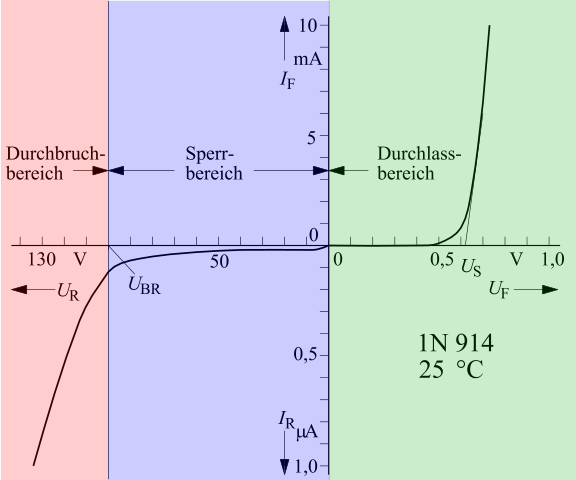
\includegraphics[scale=0.5]{Diode/Bilder/Kennlinie_Diode.png}}\\
	\subfigure[viii]{% Graphic for TeX using PGF
% Title: /home/stole/Dokumente/git/afutub-kurs/Praxisskript/Diode/Schaltungen/Z-Diode.dia
% Creator: Dia v0.97.3
% CreationDate: Mon Nov 16 20:29:49 2015
% For: stole
% \usepackage{tikz}
% The following commands are not supported in PSTricks at present
% We define them conditionally, so when they are implemented,
% this pgf file will use them.
\ifx\du\undefined
  \newlength{\du}
\fi
\setlength{\du}{15\unitlength}
\begin{tikzpicture}
\pgftransformxscale{1.000000}
\pgftransformyscale{-1.000000}
\definecolor{dialinecolor}{rgb}{0.000000, 0.000000, 0.000000}
\pgfsetstrokecolor{dialinecolor}
\definecolor{dialinecolor}{rgb}{1.000000, 1.000000, 1.000000}
\pgfsetfillcolor{dialinecolor}
\pgfsetlinewidth{0.100000\du}
\pgfsetdash{}{0pt}
\pgfsetdash{}{0pt}
\pgfsetbuttcap
\pgfsetmiterjoin
\pgfsetbuttcap
\pgfsetmiterjoin
\pgfsetdash{}{0pt}
\definecolor{dialinecolor}{rgb}{0.000000, 0.000000, 0.000000}
\pgfsetstrokecolor{dialinecolor}
\draw (5.000000\du,10.000000\du)--(5.000000\du,13.000000\du);
\pgfsetbuttcap
\pgfsetmiterjoin
\pgfsetdash{}{0pt}
\definecolor{dialinecolor}{rgb}{0.000000, 0.000000, 0.000000}
\pgfsetstrokecolor{dialinecolor}
\draw (5.000000\du,13.000000\du)--(8.000000\du,11.500000\du);
\pgfsetbuttcap
\pgfsetmiterjoin
\pgfsetdash{}{0pt}
\definecolor{dialinecolor}{rgb}{0.000000, 0.000000, 0.000000}
\pgfsetstrokecolor{dialinecolor}
\draw (5.000000\du,10.000000\du)--(8.000000\du,11.500000\du);
\pgfsetbuttcap
\pgfsetmiterjoin
\pgfsetdash{}{0pt}
\definecolor{dialinecolor}{rgb}{0.000000, 0.000000, 0.000000}
\pgfsetstrokecolor{dialinecolor}
\draw (5.000000\du,11.500000\du)--(8.000000\du,11.500000\du);
\pgfsetbuttcap
\pgfsetmiterjoin
\pgfsetdash{}{0pt}
\definecolor{dialinecolor}{rgb}{0.000000, 0.000000, 0.000000}
\pgfsetstrokecolor{dialinecolor}
\draw (8.000000\du,10.000000\du)--(8.000000\du,13.000000\du);
\pgfsetlinewidth{0.100000\du}
\pgfsetdash{}{0pt}
\pgfsetdash{}{0pt}
\pgfsetbuttcap
{
\definecolor{dialinecolor}{rgb}{0.000000, 0.000000, 0.000000}
\pgfsetfillcolor{dialinecolor}
% was here!!!
\definecolor{dialinecolor}{rgb}{0.000000, 0.000000, 0.000000}
\pgfsetstrokecolor{dialinecolor}
\draw (5.000000\du,11.500000\du)--(3.000000\du,11.500000\du);
}
\pgfsetlinewidth{0.100000\du}
\pgfsetdash{}{0pt}
\pgfsetdash{}{0pt}
\pgfsetbuttcap
{
\definecolor{dialinecolor}{rgb}{0.000000, 0.000000, 0.000000}
\pgfsetfillcolor{dialinecolor}
% was here!!!
\definecolor{dialinecolor}{rgb}{0.000000, 0.000000, 0.000000}
\pgfsetstrokecolor{dialinecolor}
\draw (8.000000\du,11.500000\du)--(10.000000\du,11.500000\du);
}
\pgfsetlinewidth{0.100000\du}
\pgfsetdash{}{0pt}
\pgfsetdash{}{0pt}
\pgfsetbuttcap
{
\definecolor{dialinecolor}{rgb}{0.000000, 0.000000, 0.000000}
\pgfsetfillcolor{dialinecolor}
% was here!!!
\definecolor{dialinecolor}{rgb}{0.000000, 0.000000, 0.000000}
\pgfsetstrokecolor{dialinecolor}
\draw (8.050000\du,13.000000\du)--(7.000000\du,13.000000\du);
}
\end{tikzpicture}
}\\
	\subfigure[iv]{% Graphic for TeX using PGF
% Title: /home/stole/Dokumente/git/afutub-kurs/Praxisskript/Diode/Schaltungen/Z-Diode_Stabilisierung.tex
% Creator: Dia v0.97.3
% CreationDate: Mon Nov 16 20:51:14 2015
% For: stole
% \usepackage{tikz}
% The following commands are not supported in PSTricks at present
% We define them conditionally, so when they are implemented,
% this pgf file will use them.
\ifx\du\undefined
  \newlength{\du}
\fi
\setlength{\du}{15\unitlength}
\begin{tikzpicture}
\pgftransformxscale{1.000000}
\pgftransformyscale{-1.000000}
\definecolor{dialinecolor}{rgb}{0.000000, 0.000000, 0.000000}
\pgfsetstrokecolor{dialinecolor}
\definecolor{dialinecolor}{rgb}{1.000000, 1.000000, 1.000000}
\pgfsetfillcolor{dialinecolor}
\pgfsetlinewidth{0.100000\du}
\pgfsetdash{}{0pt}
\pgfsetdash{}{0pt}
\pgfsetbuttcap
{
\definecolor{dialinecolor}{rgb}{0.000000, 0.000000, 0.000000}
\pgfsetfillcolor{dialinecolor}
% was here!!!
\definecolor{dialinecolor}{rgb}{0.000000, 0.000000, 0.000000}
\pgfsetstrokecolor{dialinecolor}
\draw (20.000000\du,10.000000\du)--(23.000000\du,10.000000\du);
}
\pgfsetlinewidth{0.100000\du}
\pgfsetdash{}{0pt}
\pgfsetdash{}{0pt}
\pgfsetbuttcap
{
\definecolor{dialinecolor}{rgb}{0.000000, 0.000000, 0.000000}
\pgfsetfillcolor{dialinecolor}
% was here!!!
\definecolor{dialinecolor}{rgb}{0.000000, 0.000000, 0.000000}
\pgfsetstrokecolor{dialinecolor}
\draw (20.000000\du,13.000000\du)--(23.000000\du,13.000000\du);
}
\pgfsetlinewidth{0.100000\du}
\pgfsetdash{}{0pt}
\pgfsetdash{}{0pt}
\pgfsetbuttcap
{
\definecolor{dialinecolor}{rgb}{0.000000, 0.000000, 0.000000}
\pgfsetfillcolor{dialinecolor}
% was here!!!
\definecolor{dialinecolor}{rgb}{0.000000, 0.000000, 0.000000}
\pgfsetstrokecolor{dialinecolor}
\draw (20.000000\du,13.000000\du)--(21.500000\du,10.000000\du);
}
\pgfsetlinewidth{0.100000\du}
\pgfsetdash{}{0pt}
\pgfsetdash{}{0pt}
\pgfsetbuttcap
{
\definecolor{dialinecolor}{rgb}{0.000000, 0.000000, 0.000000}
\pgfsetfillcolor{dialinecolor}
% was here!!!
\definecolor{dialinecolor}{rgb}{0.000000, 0.000000, 0.000000}
\pgfsetstrokecolor{dialinecolor}
\draw (23.000000\du,13.000000\du)--(21.500000\du,10.000000\du);
}
\pgfsetlinewidth{0.100000\du}
\pgfsetdash{}{0pt}
\pgfsetdash{}{0pt}
\pgfsetbuttcap
{
\definecolor{dialinecolor}{rgb}{0.000000, 0.000000, 0.000000}
\pgfsetfillcolor{dialinecolor}
% was here!!!
\definecolor{dialinecolor}{rgb}{0.000000, 0.000000, 0.000000}
\pgfsetstrokecolor{dialinecolor}
\draw (21.500000\du,7.000000\du)--(21.500000\du,16.000000\du);
}
\pgfsetlinewidth{0.100000\du}
\pgfsetdash{}{0pt}
\pgfsetdash{}{0pt}
\pgfsetbuttcap
{
\definecolor{dialinecolor}{rgb}{0.000000, 0.000000, 0.000000}
\pgfsetfillcolor{dialinecolor}
% was here!!!
\definecolor{dialinecolor}{rgb}{0.000000, 0.000000, 0.000000}
\pgfsetstrokecolor{dialinecolor}
\draw (20.000000\du,10.000000\du)--(20.000000\du,11.000000\du);
}
\pgfsetlinewidth{0.100000\du}
\pgfsetdash{}{0pt}
\pgfsetdash{}{0pt}
\pgfsetmiterjoin
\definecolor{dialinecolor}{rgb}{1.000000, 1.000000, 1.000000}
\pgfsetfillcolor{dialinecolor}
\fill (13.000000\du,6.000000\du)--(13.000000\du,8.000000\du)--(18.000000\du,8.000000\du)--(18.000000\du,6.000000\du)--cycle;
\definecolor{dialinecolor}{rgb}{0.000000, 0.000000, 0.000000}
\pgfsetstrokecolor{dialinecolor}
\draw (13.000000\du,6.000000\du)--(13.000000\du,8.000000\du)--(18.000000\du,8.000000\du)--(18.000000\du,6.000000\du)--cycle;
\pgfsetlinewidth{0.100000\du}
\pgfsetdash{}{0pt}
\pgfsetdash{}{0pt}
\pgfsetbuttcap
{
\definecolor{dialinecolor}{rgb}{0.000000, 0.000000, 0.000000}
\pgfsetfillcolor{dialinecolor}
% was here!!!
\definecolor{dialinecolor}{rgb}{0.000000, 0.000000, 0.000000}
\pgfsetstrokecolor{dialinecolor}
\draw (9.000000\du,7.000000\du)--(13.000000\du,7.000000\du);
}
\pgfsetlinewidth{0.100000\du}
\pgfsetdash{}{0pt}
\pgfsetdash{}{0pt}
\pgfsetbuttcap
{
\definecolor{dialinecolor}{rgb}{0.000000, 0.000000, 0.000000}
\pgfsetfillcolor{dialinecolor}
% was here!!!
\definecolor{dialinecolor}{rgb}{0.000000, 0.000000, 0.000000}
\pgfsetstrokecolor{dialinecolor}
\draw (18.000000\du,7.000000\du)--(25.000000\du,7.000000\du);
}
\pgfsetlinewidth{0.100000\du}
\pgfsetdash{}{0pt}
\pgfsetdash{}{0pt}
\pgfsetbuttcap
{
\definecolor{dialinecolor}{rgb}{0.000000, 0.000000, 0.000000}
\pgfsetfillcolor{dialinecolor}
% was here!!!
\definecolor{dialinecolor}{rgb}{0.000000, 0.000000, 0.000000}
\pgfsetstrokecolor{dialinecolor}
\draw (9.000000\du,16.000000\du)--(25.000000\du,16.000000\du);
}
\pgfsetlinewidth{0.100000\du}
\pgfsetdash{}{0pt}
\pgfsetdash{}{0pt}
\pgfsetbuttcap
{
\definecolor{dialinecolor}{rgb}{0.000000, 0.000000, 1.000000}
\pgfsetfillcolor{dialinecolor}
% was here!!!
\pgfsetarrowsend{latex}
\definecolor{dialinecolor}{rgb}{0.000000, 0.000000, 1.000000}
\pgfsetstrokecolor{dialinecolor}
\draw (9.000000\du,9.000000\du)--(9.000000\du,14.000000\du);
}
\pgfsetlinewidth{0.100000\du}
\pgfsetdash{}{0pt}
\pgfsetdash{}{0pt}
\pgfsetbuttcap
{
\definecolor{dialinecolor}{rgb}{0.000000, 0.000000, 1.000000}
\pgfsetfillcolor{dialinecolor}
% was here!!!
\pgfsetarrowsend{latex}
\definecolor{dialinecolor}{rgb}{0.000000, 0.000000, 1.000000}
\pgfsetstrokecolor{dialinecolor}
\draw (25.000000\du,9.000000\du)--(25.000000\du,14.000000\du);
}
% setfont left to latex
\definecolor{dialinecolor}{rgb}{0.000000, 0.000000, 0.000000}
\pgfsetstrokecolor{dialinecolor}
\node[anchor=west] at (7.500000\du,9.000000\du){U};
% setfont left to latex
\definecolor{dialinecolor}{rgb}{0.000000, 0.000000, 0.000000}
\pgfsetstrokecolor{dialinecolor}
\node[anchor=west] at (8.000000\du,9.200000\du){E};
% setfont left to latex
\definecolor{dialinecolor}{rgb}{0.000000, 0.000000, 0.000000}
\pgfsetstrokecolor{dialinecolor}
\node[anchor=west] at (26.000000\du,9.000000\du){U};
% setfont left to latex
\definecolor{dialinecolor}{rgb}{0.000000, 0.000000, 0.000000}
\pgfsetstrokecolor{dialinecolor}
\node[anchor=west] at (26.500000\du,9.200000\du){A};
% setfont left to latex
\definecolor{dialinecolor}{rgb}{0.000000, 0.000000, 0.000000}
\pgfsetstrokecolor{dialinecolor}
\node[anchor=west] at (26.700000\du,9.100000\du){};
% setfont left to latex
\definecolor{dialinecolor}{rgb}{0.000000, 0.000000, 0.000000}
\pgfsetstrokecolor{dialinecolor}
\node[anchor=west] at (14.000000\du,5.500000\du){R};
% setfont left to latex
\definecolor{dialinecolor}{rgb}{0.000000, 0.000000, 0.000000}
\pgfsetstrokecolor{dialinecolor}
\node[anchor=west] at (18.500000\du,10.500000\du){Vz};
\end{tikzpicture}
}
\end{figure}
}